\section{Results}
\label{sec:results}

\subsection{Baseline: isolated disk}
\label{sec:baseline}

We first verify that the model produces a stable, flat disk in the absence of tidal perturbation. Running the baseline simulation ($M_\mathrm{sat}=0$) for 3\,Gyr, we find that all rings maintain $\theta_i < 10^{-10}\,\mathrm{deg}$ throughout the integration. This confirms that the numerical scheme preserves the equilibrium state and that any warp detected in the tidal simulations is a genuine response to the satellite forcing.

\subsection{Fiducial tidal simulation}
\label{sec:fiducial}

Fig.~\ref{fig:warp_evolution} presents the fiducial simulation results ($M_\mathrm{sat}=10^{11}\,\mathrm{M}_\odot$, $i=45^\circ$, $e=0.3$).

\begin{figure*}
    \centering
    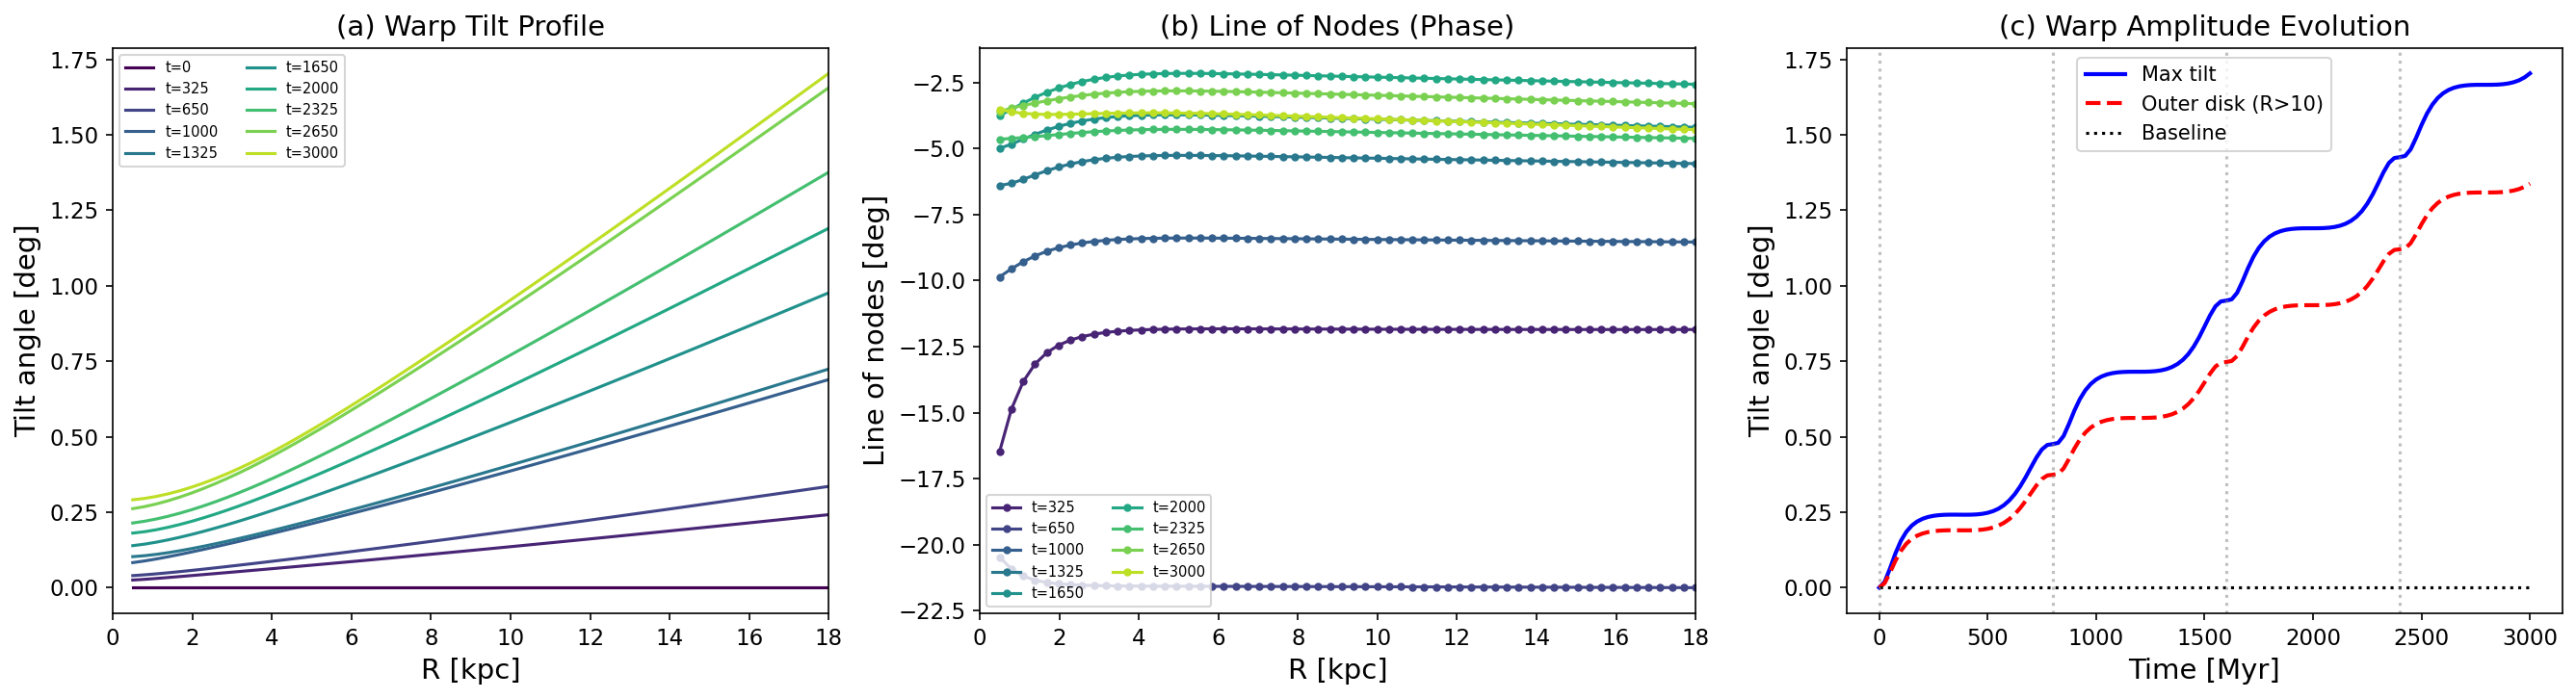
\includegraphics[width=\textwidth]{fig1_warp_evolution.png}
    \caption{Evolution of the stellar warp in the fiducial tidal simulation. \textbf{(a)} Warp tilt profile $\theta(R)$ at selected times (colour-coded). The tilt grows monotonically with radius, confirming that the outer disk is most susceptible to tidal torquing. \textbf{(b)} Line of nodes $\phi(R)$ at the same times, showing coherent precession (near-constant $\phi$ with $R$). \textbf{(c)} Time evolution of the maximum tilt (blue solid) and the mean outer-disk tilt for $R>10$\,kpc (red dashed). Vertical dotted lines mark pericentric passages ($P=800$\,Myr). The baseline (black dotted) remains flat. Note the characteristic \emph{staircase} growth pattern.}
    \label{fig:warp_evolution}
\end{figure*}

\subsubsection{Radial tilt profile}

Panel~(a) of Fig.~\ref{fig:warp_evolution} shows the tilt angle as a function of radius at ten epochs spanning $t=0$--$3000$\,Myr. Several features are noteworthy:
\begin{itemize}
    \item The tilt increases monotonically with radius at all times, consistent with the $R^2$ scaling of the tidal torque (equation~\ref{eq:T_tidal}).
    \item The inner disk ($R\lesssim4$\,kpc) remains nearly flat ($\theta < 0.1^\circ$ even at $t=3$\,Gyr), stabilized by the disk's bending stiffness provided by self-gravity coupling.
    \item At the final time, the maximum tilt is $\theta_\mathrm{max}=1.70^\circ$ at $R=18$\,kpc, and the mean outer-disk ($R>10$\,kpc) tilt is $\langle\theta\rangle_\mathrm{outer}=1.34^\circ$.
\end{itemize}

\subsubsection{Line of nodes}

Panel~(b) shows that the line of nodes is approximately constant with radius at any given time, indicating a \emph{coherent} warp without significant winding. This behaviour is characteristic of the ``modified tilt mode'' described by \citet{sparke1988}, in which the self-gravity coupling maintains coherence against the differential precession imposed by the halo.

The line of nodes precesses systematically from $\phi\approx-22^\circ$ at $t=325$\,Myr to $\phi\approx-2^\circ$ at $t=3000$\,Myr, yielding a mean precession rate of ${\sim}7\,\mathrm{deg\,Gyr^{-1}}$.

\subsubsection{Staircase growth}

Panel~(c) reveals the most distinctive feature of the tidal warp: the amplitude grows in a \emph{staircase pattern}, with each step corresponding to a pericentric passage of the satellite ($P=800$\,Myr, marked by vertical lines). Between passages, the warp amplitude plateaus. This demonstrates that warp growth is impulsive -- driven by the concentrated tidal torque near pericentre -- rather than a slow, continuous process. Each passage delivers a discrete ``kick'' that incrementally tilts the outer rings.

\subsection{3D morphology}
\label{sec:morphology}

Figs~\ref{fig:3d_warp} and~\ref{fig:disk_views} show the warped disk morphology at selected epochs. The 3D scatter plot (Fig.~\ref{fig:3d_warp}) reveals a progressively developing integral-sign (S-shaped) warp, with the outer disk bending above and below the midplane on opposite sides. The edge-on density map (Fig.~\ref{fig:disk_views}, bottom row) makes the warp directly visible as a systematic bending of the disk plane at large radii.

\begin{figure*}
    \centering
    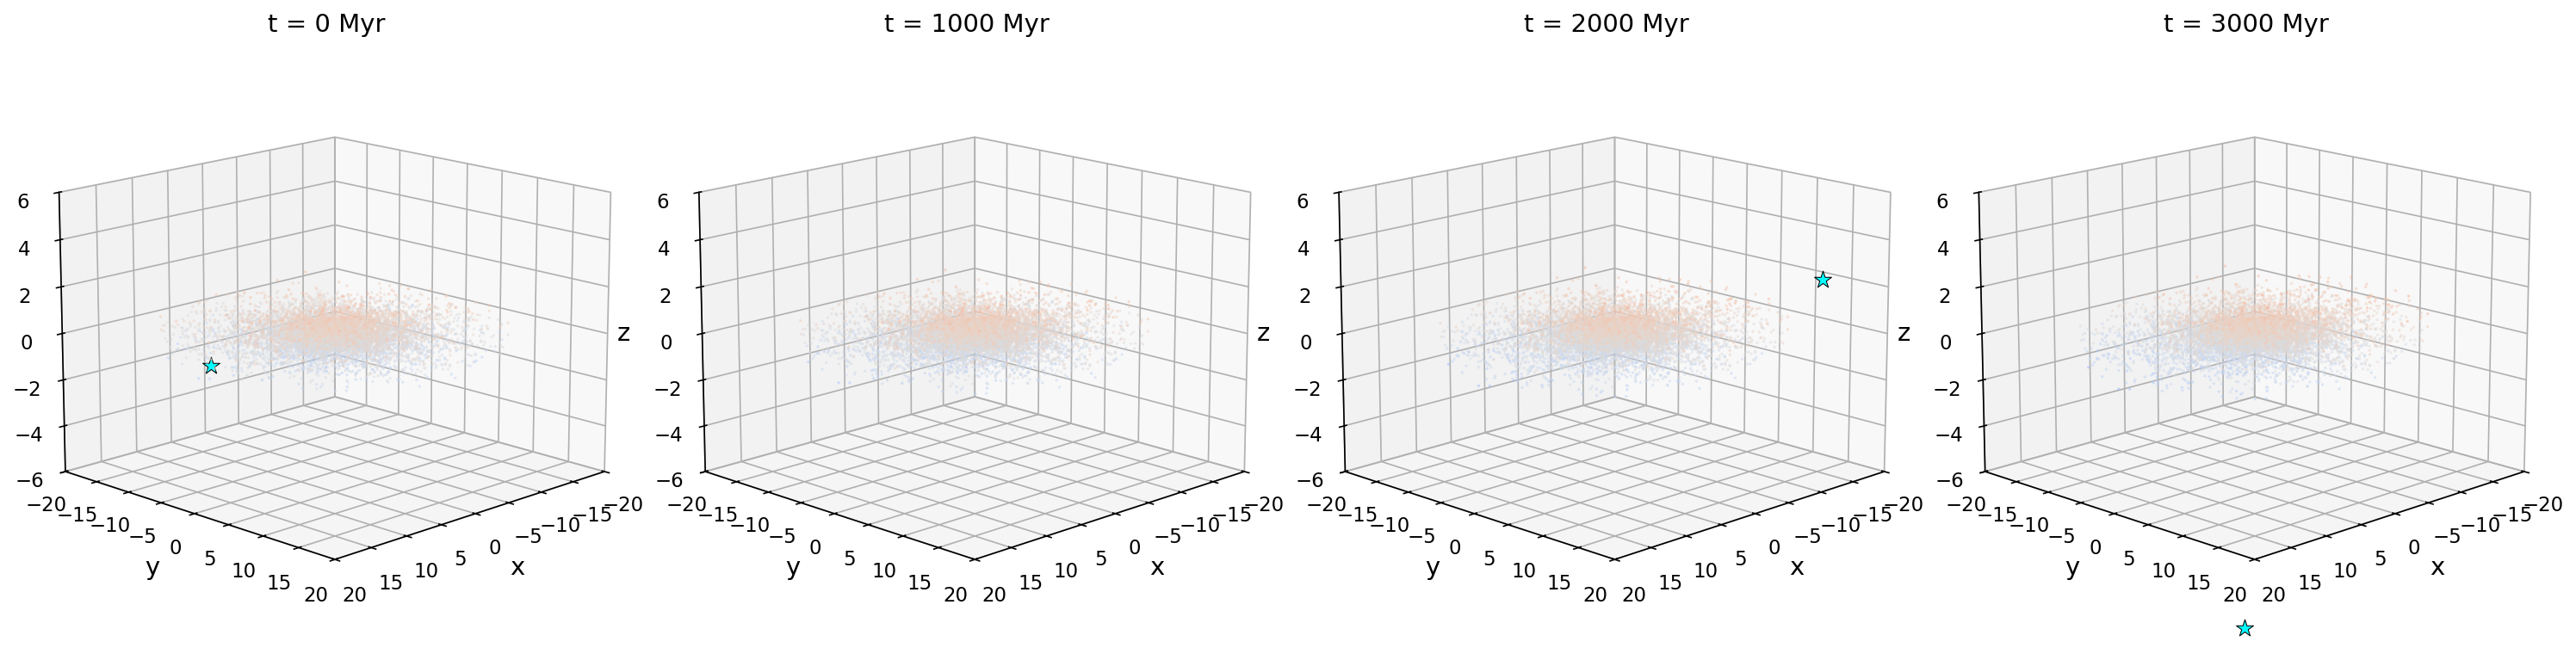
\includegraphics[width=\textwidth]{fig2_3d_warp.png}
    \caption{Three-dimensional visualization of the warped disk at $t=0$, 1000, 2000, and 3000\,Myr. Particles are colour-coded by height $z$ (blue: below midplane; red: above). The cyan star marks the satellite position. The progressive development of an S-shaped warp is clearly visible.}
    \label{fig:3d_warp}
\end{figure*}

\begin{figure*}
    \centering
    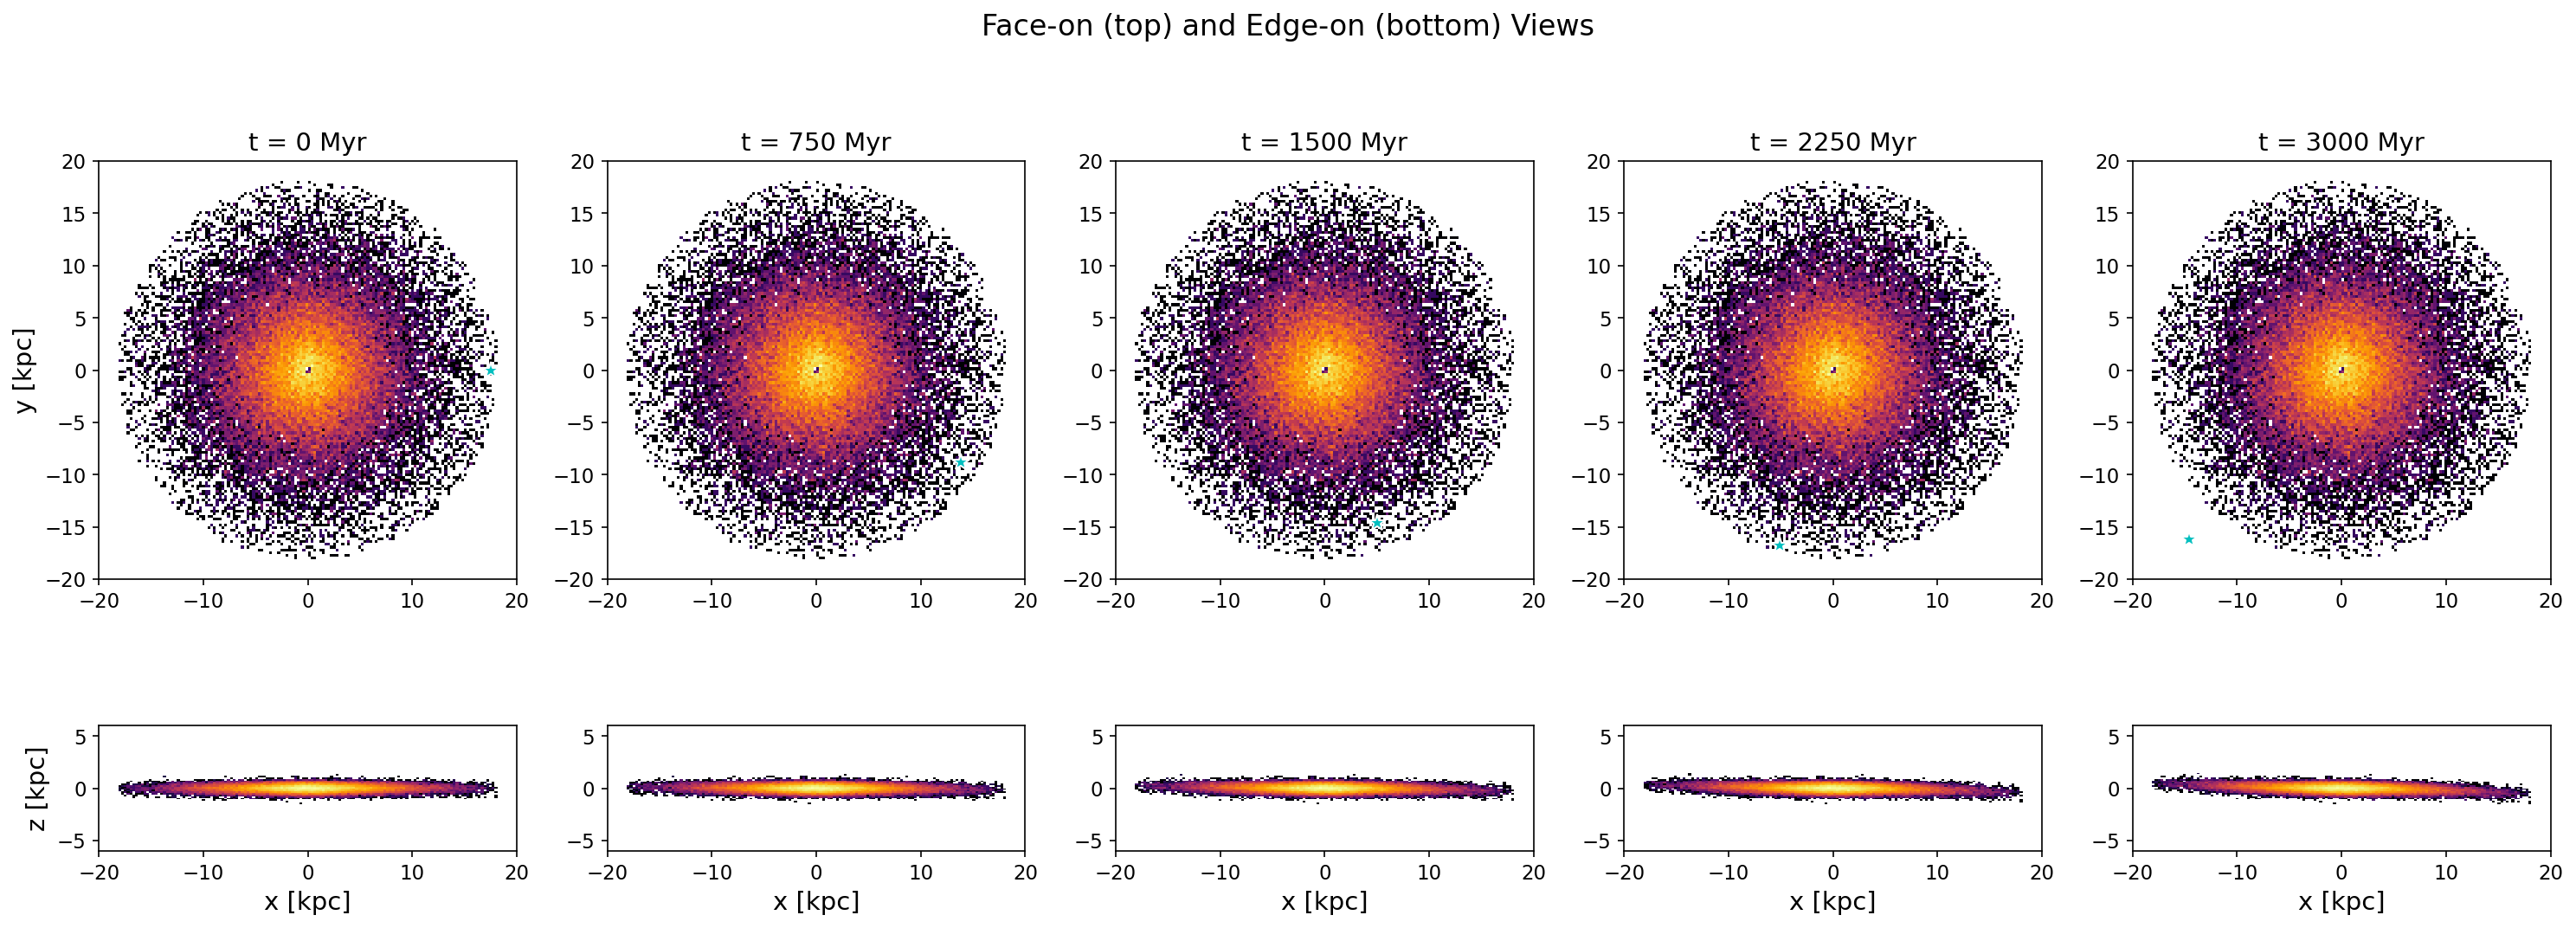
\includegraphics[width=\textwidth]{fig3_disk_views.png}
    \caption{Face-on (top) and edge-on (bottom) projected density maps at five epochs. The satellite position is marked by a cyan star. The edge-on views reveal the characteristic warp bending of the outer disk.}
    \label{fig:disk_views}
\end{figure*}

\subsection{Torque decomposition}
\label{sec:torques}

Fig.~\ref{fig:torque} decomposes the three torque components at $t=3000$\,Myr, when the warp is fully developed.

\begin{figure*}
    \centering
    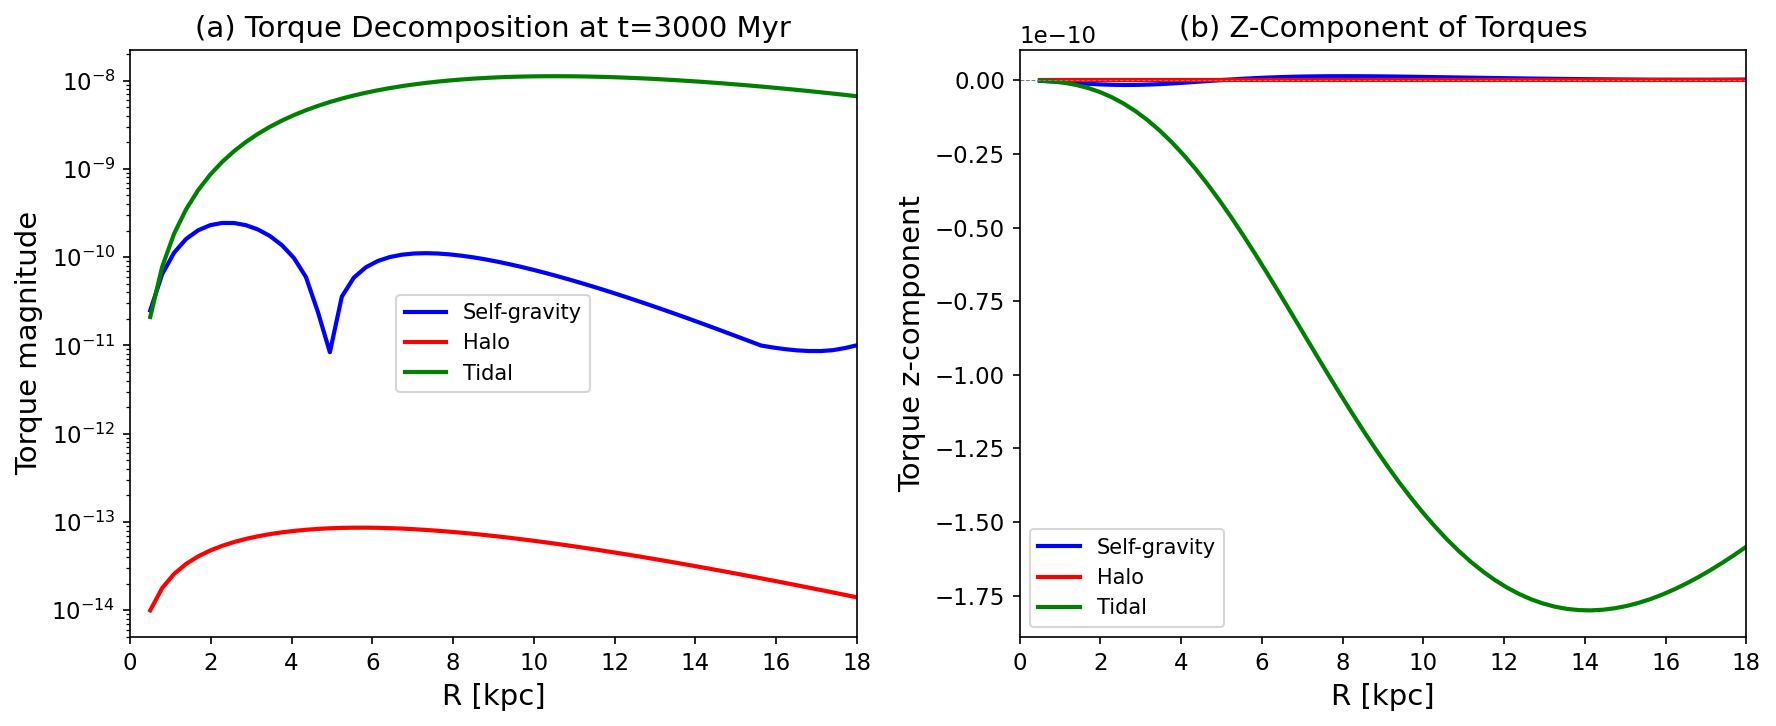
\includegraphics[width=\textwidth]{fig7_torque_decomposition.png}
    \caption{Torque decomposition at $t=3000$\,Myr. \textbf{(a)} Torque magnitude versus galactocentric radius on a logarithmic scale. The tidal torque (green) dominates at all $R>2$\,kpc, exceeding self-gravity (blue) by 1--3 orders of magnitude and the halo torque (red) by ${\sim}3$ orders of magnitude. \textbf{(b)} The $z$-component of each torque. The tidal $z$-torque scales as ${\sim}R^2$ and is the primary driver of the warp.}
    \label{fig:torque}
\end{figure*}

Panel~(a) shows the torque magnitudes on a logarithmic scale. The tidal torque dominates at all radii $R>2$\,kpc, exceeding the disk self-gravity torque by 1--3 orders of magnitude. The self-gravity torque shows a characteristic bump at $R\sim3$--$5$\,kpc, corresponding to the peak of the disk surface density ($R_d=3.5$\,kpc). The halo torque is subdominant everywhere by approximately 3 orders of magnitude.

Panel~(b) shows the $z$-component of each torque. The tidal $z$-torque has a smooth profile scaling approximately as $R^2$ and is the direct driver of the vertical bending. The self-gravity and halo contributions are negligible on this scale.

This torque hierarchy explains the insensitivity of the warp to halo flattening (Section~\ref{sec:params}): the halo torque is simply too weak relative to the tidal forcing to influence the warp amplitude.

\subsection{Parameter study}
\label{sec:params}

We conduct three parameter studies, varying the satellite mass, orbital inclination, and halo axis ratio individually while holding all other parameters at their fiducial values.

\subsubsection{Satellite mass}
\label{sec:param_mass}

\begin{figure*}
    \centering
    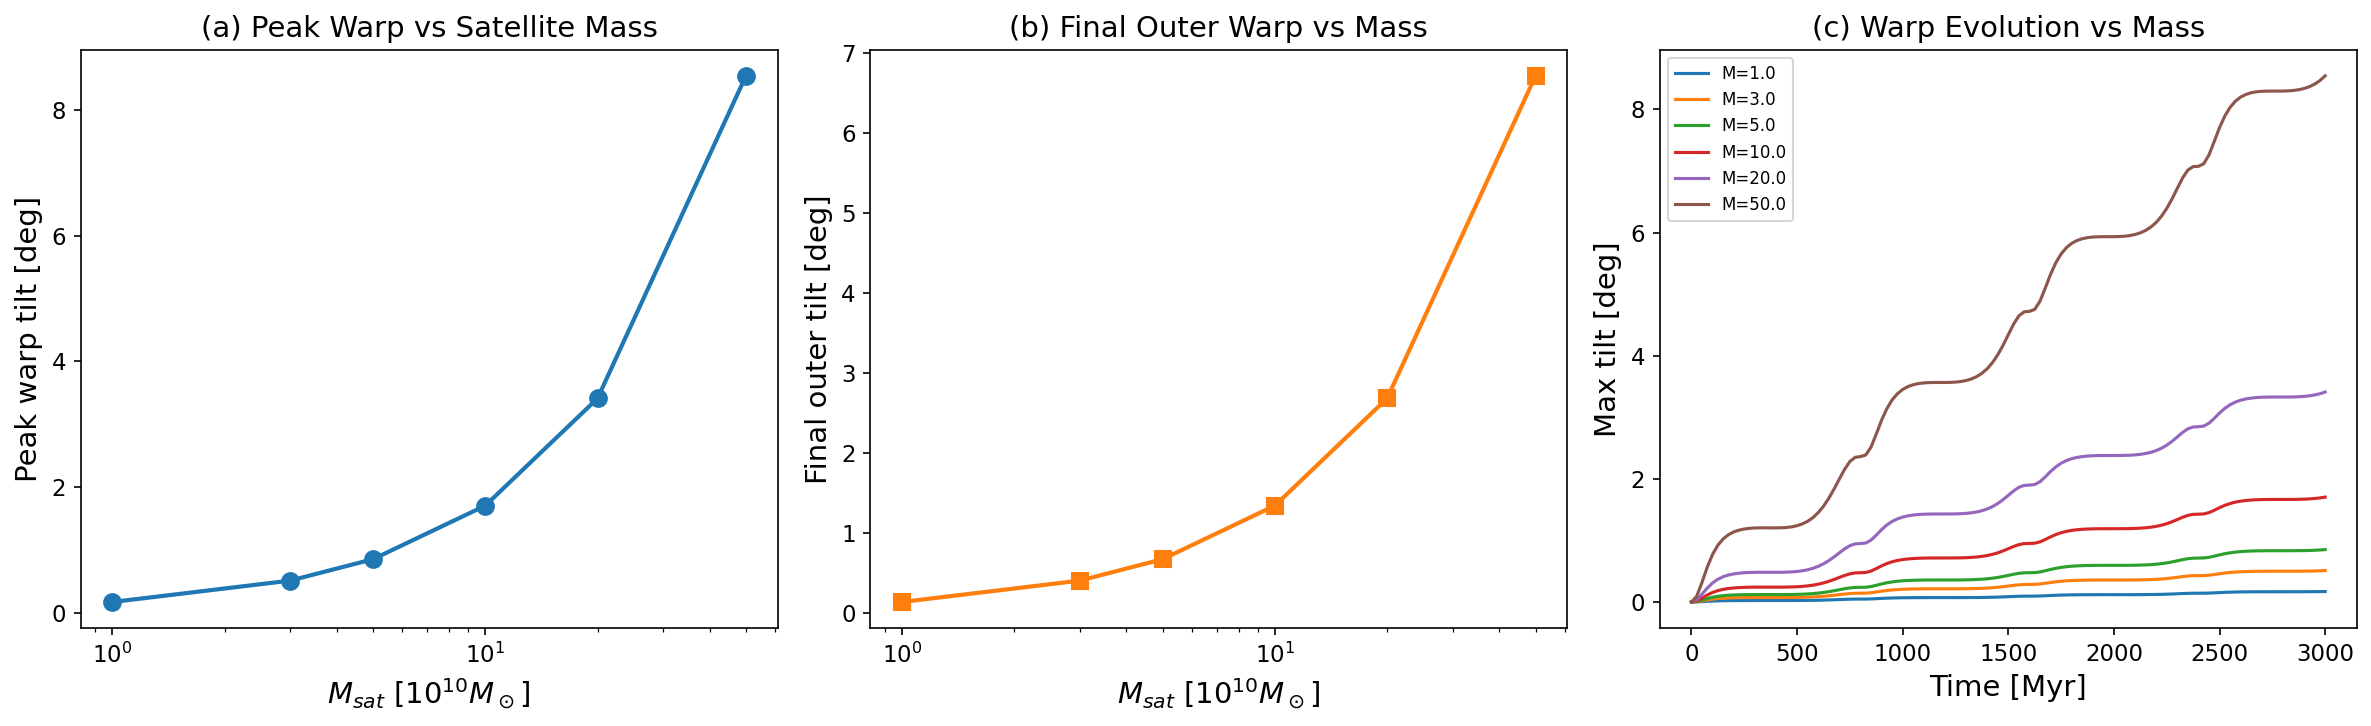
\includegraphics[width=\textwidth]{fig4_param_Msat.png}
    \caption{Parameter study: satellite mass. \textbf{(a)} Peak warp tilt versus $M_\mathrm{sat}$ (log scale). \textbf{(b)} Final outer-disk tilt versus $M_\mathrm{sat}$. \textbf{(c)} Warp amplitude evolution for each mass. The warp amplitude scales approximately linearly with $M_\mathrm{sat}$.}
    \label{fig:param_mass}
\end{figure*}

Fig.~\ref{fig:param_mass} shows the warp amplitude as a function of satellite mass for $M_\mathrm{sat} = 1, 3, 5, 10, 20, 50 \times 10^{10}\,\mathrm{M}_\odot$.

The peak warp tilt scales approximately linearly with $M_\mathrm{sat}$ over two orders of magnitude: from $0.17^\circ$ at $M_\mathrm{sat}=10^{10}\,\mathrm{M}_\odot$ to $8.55^\circ$ at $M_\mathrm{sat}=5\times10^{11}\,\mathrm{M}_\odot$. This linear scaling is expected analytically from equation~(\ref{eq:T_tidal}), where $T^\mathrm{tidal}\propto M_\mathrm{sat}$.

The time evolution panel~(c) shows that all masses produce the same staircase growth pattern, with larger satellites generating higher steps. The warp onset is also earlier for more massive perturbers, as the first pericentric passage delivers a proportionally larger kick.

Table~\ref{tab:results_mass} summarizes the key metrics.

\begin{table}
    \centering
    \caption{Peak warp tilt as a function of satellite mass.}
    \label{tab:results_mass}
    \begin{tabular}{ccc}
        \toprule
        $M_\mathrm{sat}$ [$10^{10}\,\mathrm{M}_\odot$] & Peak tilt [deg] & Final outer tilt [deg] \\
        \midrule
        1.0  & 0.17 & 0.13 \\
        3.0  & 0.51 & 0.40 \\
        5.0  & 0.85 & 0.67 \\
        10.0 & 1.70 & 1.34 \\
        20.0 & 3.41 & 2.68 \\
        50.0 & 8.55 & 6.71 \\
        \bottomrule
    \end{tabular}
\end{table}

\subsubsection{Orbital inclination}
\label{sec:param_incl}

\begin{figure*}
    \centering
    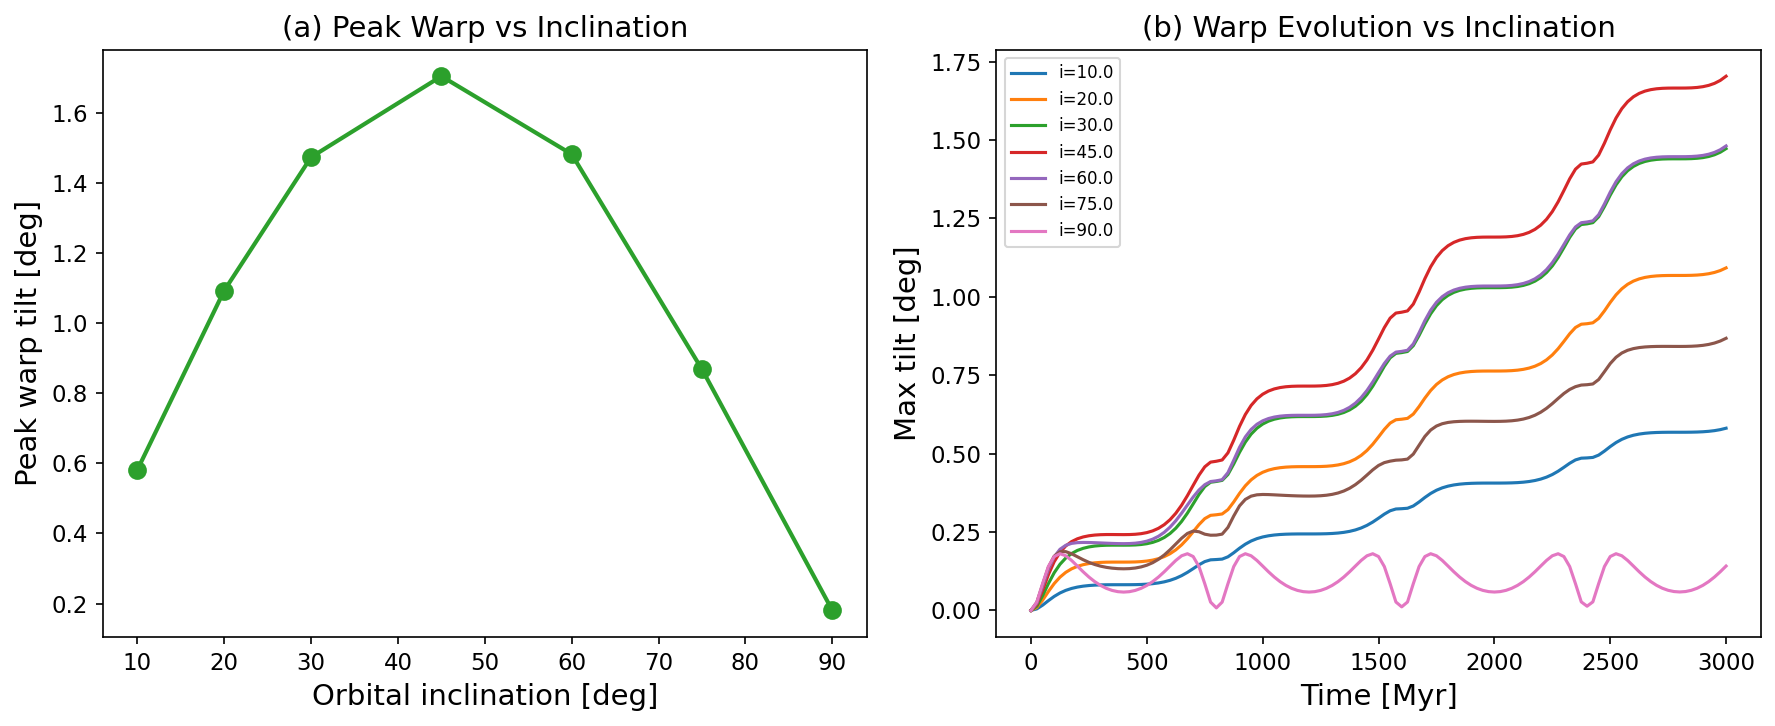
\includegraphics[width=\textwidth]{fig5_param_inclination.png}
    \caption{Parameter study: orbital inclination. \textbf{(a)} Peak warp tilt versus inclination. The curve peaks at $i\approx45^\circ$, consistent with a $\sin 2i$ dependence. \textbf{(b)} Warp amplitude evolution for each inclination. The $i=90^\circ$ case shows oscillatory behaviour.}
    \label{fig:param_incl}
\end{figure*}

Fig.~\ref{fig:param_incl} shows the warp amplitude for orbital inclinations $i = 10^\circ$, $20^\circ$, $30^\circ$, $45^\circ$, $60^\circ$, $75^\circ$, and $90^\circ$.

The peak warp tilt is maximized at $i=45^\circ$ ($1.70^\circ$) and drops to $0.18^\circ$ at $i=90^\circ$. This behaviour reflects the $\sin 2i$ dependence of the tidal torque's vertical component. Physically, the tidal torque requires the satellite to have a component of its position vector both along and perpendicular to the disk plane. At $i=0^\circ$ (coplanar orbit), there is no out-of-plane forcing; at $i=90^\circ$ (polar orbit), the time-averaged vertical torque nearly cancels because the satellite spends equal time above and below the disk.

The time evolution [panel~(b)] reveals qualitatively distinct behaviour at extreme inclinations. The $i=90^\circ$ orbit produces an \emph{oscillatory} warp, with the tilt oscillating around ${\sim}0.1$--$0.2^\circ$ as the torque reverses sign each half-orbit. In contrast, intermediate inclinations ($30^\circ$--$60^\circ$) produce monotonically growing warps with clear staircase structure.

Table~\ref{tab:results_incl} summarizes the inclination dependence.

\begin{table}
    \centering
    \caption{Peak warp tilt as a function of orbital inclination.}
    \label{tab:results_incl}
    \begin{tabular}{cccc}
        \toprule
        $i$ [deg] & Peak tilt [deg] & $\sin 2i$ & Ratio \\
        \midrule
        10 & 0.59 & 0.342 & 1.72 \\
        20 & 1.09 & 0.643 & 1.70 \\
        30 & 1.47 & 0.866 & 1.70 \\
        45 & 1.70 & 1.000 & 1.70 \\
        60 & 1.48 & 0.866 & 1.71 \\
        75 & 0.87 & 0.500 & 1.74 \\
        90 & 0.18 & 0.000 & --- \\
        \bottomrule
    \end{tabular}
    \begin{minipage}{\columnwidth}
    \vspace{0.1cm}
    \footnotesize{Note: The ``Ratio'' column is $\theta_\mathrm{peak}/\sin 2i$, showing approximate constancy for $i\neq90^\circ$, confirming the $\sin 2i$ scaling.}
    \end{minipage}
\end{table}

\subsubsection{Halo flattening}
\label{sec:param_qhalo}

\begin{figure*}
    \centering
    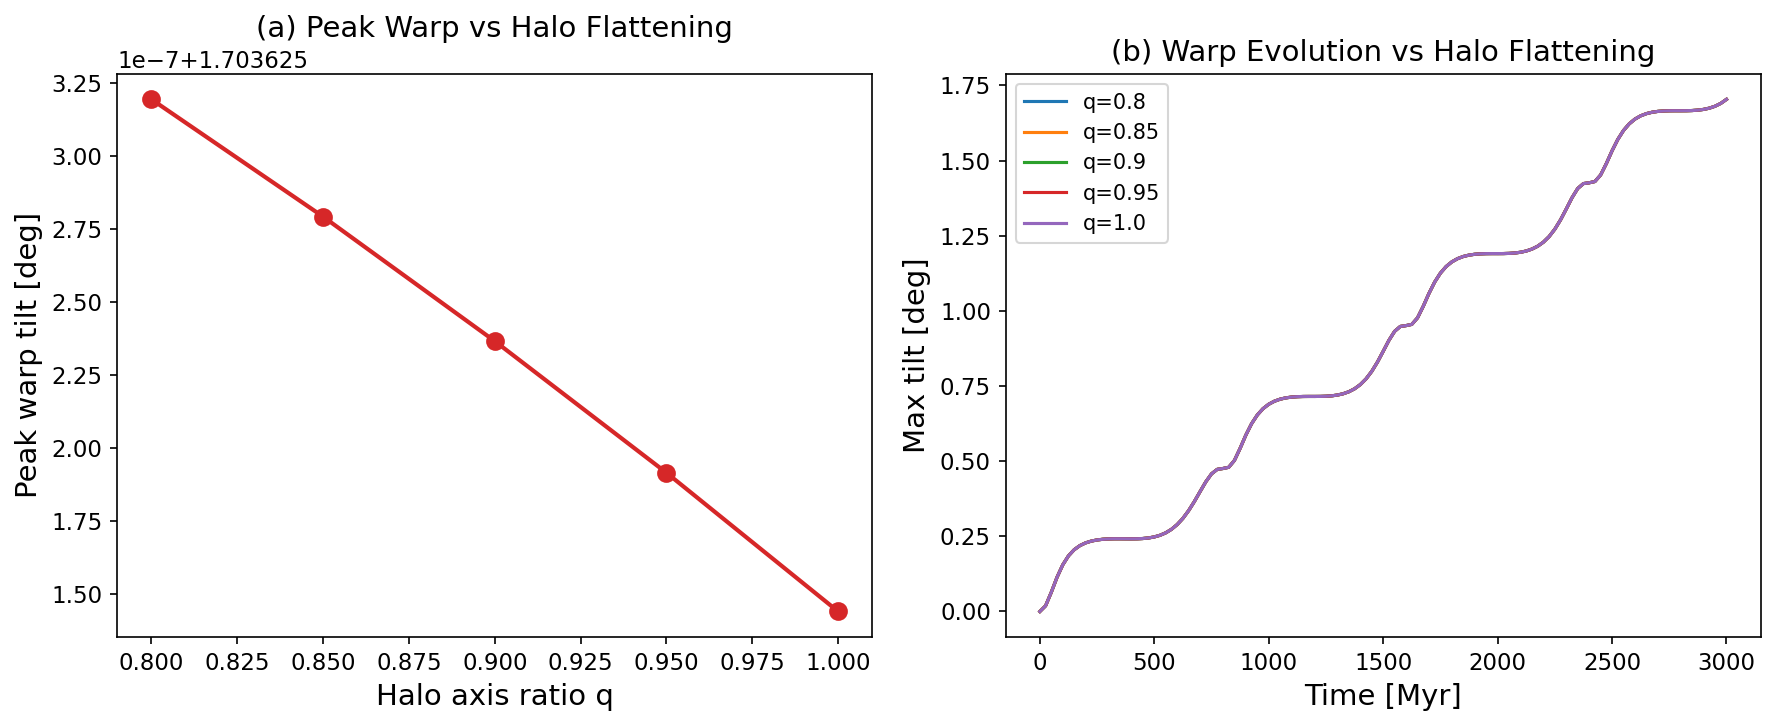
\includegraphics[width=\textwidth]{fig6_param_qhalo.png}
    \caption{Parameter study: halo axis ratio $q$. \textbf{(a)} Peak warp tilt versus $q$. \textbf{(b)} Warp evolution for each $q$ value. No significant dependence is found, as the tidal torque overwhelms the halo torque.}
    \label{fig:param_qhalo}
\end{figure*}

Fig.~\ref{fig:param_qhalo} shows the warp amplitude for halo axis ratios $q = 0.80$, $0.85$, $0.90$, $0.95$, and $1.00$ (spherical). No significant variation is detected: all five runs produce identical peak tilts of $1.70^\circ$ and identical outer-disk tilts of $1.34^\circ$.

This null result is a direct consequence of the torque hierarchy (Section~\ref{sec:torques}): the halo torque is ${\sim}3$ orders of magnitude weaker than the tidal torque, so varying $q$ (and hence $\nu_p^2 \propto 1-q^2$) has no appreciable effect on the warp amplitude. We emphasize that this insensitivity is specific to the regime of strong tidal forcing; for isolated disks or weak perturbers, the halo torque would control the warp's long-term precession and winding behaviour.
